\documentclass[conference]{IEEEtran}
\IEEEoverridecommandlockouts
\usepackage{cite}
\usepackage{amsmath,amssymb,amsfonts}
\usepackage{algorithmic}
\usepackage{graphicx}
\usepackage{textcomp}
\usepackage{xcolor}
\usepackage{url}
\usepackage{subcaption}
\def\BibTeX{{\rm B\kern-.05em{\sc i\kern-.025em b}\kern-.08em
    T\kern-.1667em\lower.7ex\hbox{E}\kern-.125emX}}

\begin{document}

\title{Vision-Only Autonomous Drone Inspection with SAM 3 Identification, Bearing-Only Triangulation, and Hybrid 3D Reconstruction in Simulation}

\author{\IEEEauthorblockN{Mohamed Gallai}
\IEEEauthorblockA{\textit{Department of Electrical and Computer Engineering} \\
\textit{Binghamton University}\\
Binghamton, NY, USA \\
mgallai@binghamton.edu}
}

\maketitle

\begin{abstract}
We present an autonomous target-inspection pipeline for a simulated
unmanned aerial vehicle (UAV). Given only the natural-language name
of an object, the system searches a populated room, identifies the
target without fiducial markers or an object-position prior, orbits
it twice at two altitudes, and produces four 3D outputs:
target-only and full-scene 3D Gaussian Splatting reconstructions, a
Depth Anything~3 (DA3) colored point cloud, and an Open3D Poisson
triangle mesh. The pipeline is autonomous with respect to target
discovery and mission execution, while the vehicle self-pose is
provided by Gazebo ground truth in simulation. The system runs
end-to-end in approximately 20 minutes per target on an 8\,GB
consumer GPU. Object identification is performed with SAM~3, and
object localization is solved using bearing-only triangulation
across multi-view detections, with a $25^{\circ}$ angular-spread
gate that detects near-parallel-ray degeneracy. We evaluate the
system by shuffling five test objects among five canonical
positions at launch, so the drone has no SDF position prior and
must visually rediscover each target. Across five targets and one
moved-target test, four of six cases localize below 1\,m, five of
six are within 1.06\,m, and the main outlier is the bench at
1.91\,m. The work evolved away from the initial AprilTag and COLMAP
proposal toward a SAM~3, DA3, and splatfacto hybrid, and the
results suggest that an open-source ROS\,2 and Gazebo stack can
support modern foundation-vision models in a closed-loop simulation
pipeline when the scene assets are chosen carefully.
\end{abstract}

\begin{IEEEkeywords}
autonomous drone, foundation models, SAM 3, 3D Gaussian Splatting,
Depth Anything 3, ROS 2, Gazebo, bearing-only triangulation,
3D reconstruction, vision-language model
\end{IEEEkeywords}

\section{Introduction}

Robotic 3D inspection of arbitrary, user-specified objects sits at the
intersection of three traditionally separate problems: \emph{recognition}
(``find the fire hydrant''), \emph{localization in the world}
(``where is it in metric coordinates?''), and \emph{geometry capture}
(``produce a 3D model suitable for inspection''). Until
recently, these were typically solved by attaching a fiducial marker
to the target (e.g., AprilTag \cite{olson2011apriltag},
\cite{wang2016apriltag2}), running offline structure-from-motion such
as COLMAP \cite{schonberger2016sfm}, \cite{schonberger2016mvs} on a
manually-piloted image set, and treating localization as a separate
SLAM problem. Each step required calibration or human intervention;
none generalized to a new object class without re-engineering.

In the last two years, three capability shifts have made this type of
vision-centered simulation pipeline practical:
\begin{itemize}
    \item \textbf{Open-vocabulary segmentation} via foundation models
    such as SAM \cite{kirillov2023sam}, which segments any object
    given a point or box prompt, and SAM 3 \cite{carion2025sam3},
    which extends this to short text concept prompts so that object
    categories can be detected and segmented without training a
    task-specific detector.
    \item \textbf{Photorealistic 3D representations} from photo sets:
    3D Gaussian Splatting \cite{kerbl2023_3dgs} supports high-quality,
    real-time novel-view rendering and is available through
    nerfstudio's \texttt{splatfacto} implementation
    \cite{tancik2023nerfstudio}.
    \item \textbf{Robust monocular and multi-view depth estimation}:
    Depth Anything \cite{yang2024depthanything} provided strong
    monocular depth from a single image, and Depth Anything 3 (DA3)
    \cite{lin2025da3} extends the family to multi-view inputs by
    jointly predicting spatially consistent depth and refining camera
    extrinsics across the input set.
\end{itemize}

This work integrates these advances into a single autonomy pipeline
running on top of ROS\,2 Jazzy \cite{macenski2022ros2} and Gazebo Sim
\cite{koenig2004gazebo}. The drone receives only a text prompt
(or a transcribed voice command, or an output of a local large
language model), executes a structured search of an unknown room,
visually identifies the requested object, orbits it twice at two
altitudes, and emits four 3D output files. The localization step does
not rely on any prior knowledge of object positions; instead, the
drone fuses multi-view bearing measurements through a closed-form
least-squares triangulation. To verify that the system genuinely
relies on visual target discovery, we randomize object placement at
every launch: five canonical positions are fixed, but the assignment
of each physical object to a slot is shuffled, and that assignment is
not exposed to the mission node.

\subsection{Evolution from the original proposal}

The original project proposal \cite{gallai_proposal_2026} specified an
AprilTag fiducial marker for target detection and COLMAP for offline
photogrammetric reconstruction. Both choices were dropped during
implementation in favor of more general approaches. AprilTag forces a
marker to be physically placed on the target, undermining the
``vision-only autonomy'' claim and limiting the system to a single
known marker per mission. SAM 3 replaces this marker requirement with open-vocabulary
segmentation: the same pipeline can be launched with any of the five
test-object names without changing the detector. Similarly, the
structure-from-motion (SfM) stage of a COLMAP-style pipeline depends
on stable feature matching, which is known to be challenging on the
smooth, low-texture primitive surfaces present in our scene. The
DA3\,+\,splatfacto path was therefore a better fit for our simulator
assets and for the desired combination of colored geometry and
novel-view rendering.

\subsection{Response to proposal feedback on photorealism}

A reviewer noted that Gazebo Sim is not very photorealistic and may
not support SAM 3's image quality requirements. We acknowledge this
concern and address it in two ways. First, we empirically verified
that Gazebo's \texttt{ogre2} renderer, when paired with carefully
chosen asset materials and lighting, produces images on which SAM 3
detects the target reliably in our controlled scene (scores of
0.85 for the plant and 0.94 for the fire hydrant; see
Section~\ref{sec:results}). Second, we replaced three Gazebo-Fuel
community models that SAM 3 did \emph{not} recognize with hand-built
primitive geometries; after this change, the same object names became
reliably segmentable. This does not make Gazebo generally
photorealistic, but it shows that asset choice alone can make the
simulator usable for this closed-loop perception experiment.

The reviewer also suggested SAM 3D from Meta as an alternative to
classical photogrammetry. SAM 3D estimates a 3D shape from a single
image and mask, which is well-suited to instant 3D-from-photograph
applications but does not directly use the multi-view orbit collected
by the drone. We instead use the multi-view DA3 model
\cite{lin2025da3}, which refines per-frame geometry and camera-pose
consistency across the captured view set. The resulting point cloud
is spatially coherent across all 48 selected frames; its metric
accuracy is inherited from the simulator scale and camera-pose
recording and should be validated quantitatively in future work.
splatfacto adds a separate novel-view-rendering representation from
the same image set.

\subsection{Contributions}

This paper presents the following contributions:
\begin{enumerate}
    \item A full ROS\,2 / Gazebo / SAM 3 / DA3 / splatfacto autonomy
    pipeline with end-to-end runtime under 20 minutes on an 8\,GB
    consumer GPU.
    \item A bearing-only triangulation algorithm for multi-view
    object localization, with a closed-form least-squares solution
    and a $25^{\circ}$ angular-spread gate to detect and reject
    parallel-ray degeneracy. The gate triggers a fallback to a
    score-weighted spatial median.
    \item A scene-randomization mechanism that tests whether the
    system is genuinely vision-driven: by shuffling five objects among
    five canonical slots at every launch and hiding the assignment
    from \texttt{mission\_node}, we eliminate the possibility of an
    SDF position prior leaking into the pipeline.
    \item An empirical evaluation across five targets and one moved-target
    test, with four of six localization errors below 1\,m and five
    of six within 1.06\,m, without any target-position prior.
    \item A virtual-gimbal pitch correction during orbit that
    keeps the target near image-center across both orbit
    altitudes, preventing tracker drift to nearby distractors.
\end{enumerate}

\section{Related Work}

\subsection{Visual fiducials and open-vocabulary segmentation}

AprilTag \cite{olson2011apriltag} introduced a robust, low-cost
fiducial marker system that has become a standard tool for autonomous
robot localization. Subsequent work \cite{wang2016apriltag2} improved
detection efficiency. While reliable, fiducials require physical
placement on the target and identify only known marker IDs. The
Segment Anything Model (SAM) \cite{kirillov2023sam} eliminated the
need for class-specific training: SAM produces high-quality
segmentation masks for any object given a point or box prompt. Subsequent
work extended segmentation pipelines toward text grounding and video
tracking. SAM 3 \cite{carion2025sam3} introduces promptable concept
segmentation, in which short noun phrases, image exemplars, or both
can be used to detect, segment, and track matching object instances.
In this project, \texttt{sam3\_detector} uses the SAM 3 semantic
segmentation interface for image-frame target masks.

\subsection{3D reconstruction from images}

Classical structure-from-motion pipelines such as COLMAP
\cite{schonberger2016sfm}, \cite{schonberger2016mvs} dominated 3D
reconstruction for a decade but require well-textured surfaces and
tend to fail on simulated assets with smooth materials.
Neural radiance fields (NeRF) \cite{mildenhall2020nerf} introduced
volumetric rendering for novel view synthesis but at very high
training cost. 3D Gaussian Splatting \cite{kerbl2023_3dgs} replaced
volumetric integration with explicit anisotropic Gaussian primitives,
achieving real-time rendering and dramatically faster training. The
nerfstudio framework's \texttt{splatfacto}
\cite{tancik2023nerfstudio} provides a turnkey 3DGS implementation
which we use here.

For monocular depth estimation, the Depth Anything family
\cite{yang2024depthanything} demonstrated that a vision transformer
trained on 62\,M images plus 1.5\,M depth labels can predict
high-quality depth on arbitrary scenes. Depth Anything 3 (DA3)
\cite{lin2025da3}, used in this work, extends the family to
multi-view inputs and jointly refines per-frame depth and camera
extrinsics across the input set, which is useful for fusing the orbit
image set into a single colored point cloud.

\subsection{UAV planning for reconstruction}

The UAV photogrammetry literature has long emphasized that
reconstruction quality depends on capture pattern.
Zhang et al.~\cite{zhang2020uav_planning} demonstrated that
self-occlusion makes simple orbit patterns insufficient and motivated
multi-altitude capture. Our two-ring orbit (low + high) follows this
recommendation. Recent work on adaptive view planning
\cite{smith2018adaptive_view} optimizes views to maximize information
gain; we leave adaptive planning as future work and adopt a
deterministic two-altitude orbit because it is sufficient for
our object scale and orbit radius.

\subsection{ROS 2 and Gazebo for UAV simulation}

ROS\,2 \cite{macenski2022ros2} is the de facto open-source robot
middleware. Gazebo Sim \cite{koenig2004gazebo} provides physics,
sensors, and rendering for robot simulation. The
\texttt{ros\_gz\_bridge} translates between Gazebo's native
transport and ROS\,2 topics, enabling foundation-model-based
perception code (which expects ROS topics) to consume simulated
camera streams transparently. We selected Gazebo over alternatives
such as Isaac Sim and AirSim for this specific project because
Gazebo provides native ROS\,2 integration, simple SDF/XML scene
authoring, deterministic kinematic pose control, and reliable
operation on the available 8\,GB GPU. This choice was practical
rather than universal: current Isaac Sim documentation lists 16\,GB
of VRAM as the minimum specification for the 5.1 workstation
workflow and warns that lower-VRAM GPUs may be insufficient for
complex rendering workloads \cite{nvidia_isaac_req}, while the
official Microsoft AirSim release page lists v1.8.1 (2022) as the
most recent release \cite{airsim_releases}.

\section{System Architecture}
\label{sec:architecture}

\begin{figure*}[!t]
\centerline{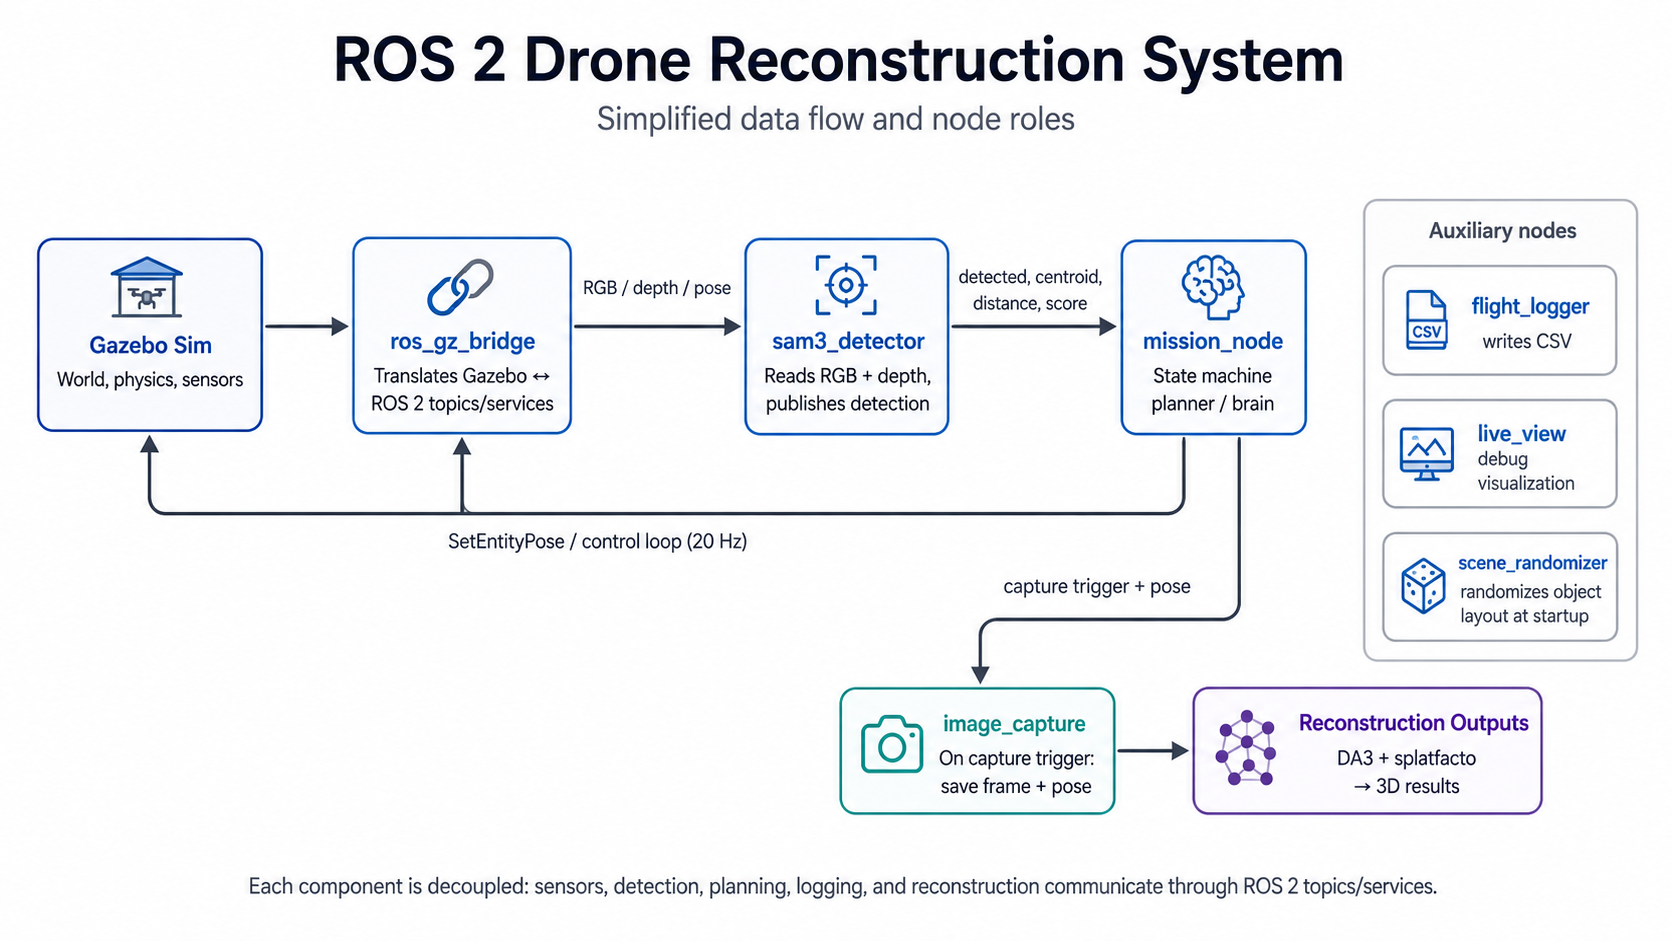
\includegraphics[width=0.95\textwidth]{figures/architecture.png}}
\caption{Simplified ROS\,2 data flow. Five primary nodes plus three
auxiliaries (\texttt{flight\_logger}, \texttt{live\_view},
\texttt{scene\_randomizer}) communicate via topics and services.
The kinematic teleport loop runs at 20\,Hz; SAM 3 inference runs at
approximately 2\,Hz. No SLAM is used: the drone uses Gazebo's
ground-truth vehicle pose, while the target position is estimated
from vision-based detections.}
\label{fig:architecture}
\end{figure*}

The system comprises five primary ROS\,2 nodes plus three auxiliary
nodes (Fig.~\ref{fig:architecture}). \texttt{mission\_node} is the
state machine and motion planner, owning all decisions about where
the drone goes next. \texttt{sam3\_detector} hosts the SAM 3 model on
GPU and publishes per-frame detection results. \texttt{image\_capture}
buffers the camera stream and saves frames plus poses to disk on
trigger. \texttt{ros\_gz\_bridge} translates between Gazebo's native
transport and ROS\,2. The auxiliaries are \texttt{scene\_randomizer}
(one-shot at startup, shuffles object positions),
\texttt{flight\_logger} (writes per-tick CSV telemetry), and
\texttt{live\_view} (a custom OpenCV window that overlays the SAM 3
mask on the live camera stream).

\subsection{Why no SLAM?}

The mission node uses Gazebo's ground-truth drone pose obtained via
the bridged \texttt{/world/recon\_world/set\_pose} service. This means
that the project evaluates autonomous target discovery, target
localization, and image capture, but it does \emph{not} evaluate
vehicle state estimation. SLAM would be required for hardware
deployment or for a simulation study focused on drone self-localization;
here, using simulator ground truth keeps the experiment focused on the
unknown target object's position.

\subsection{Why kinematic teleport, not velocity-controlled flight}

The drone is driven via direct \texttt{SetEntityPose} writes every
50\,ms (kinematic mode) rather than through \texttt{Twist} commands on
\texttt{/cmd\_vel} (\texttt{velocity\_kinematic} mode), although both
modes are implemented. The motivation is splat-training data quality.
3D Gaussian Splatting back-projects each captured image through its
associated camera pose to compute reprojection error; if the pose
recorded in \texttt{transforms.json} disagrees with the camera's actual
pose at capture time by even a few centimeters, the optimizer cannot
fully reconcile the contradiction and the result can become a visibly
smeared splat with floater artifacts. In velocity-controlled flight,
the closed-loop controller tracks its commanded waypoint with
5--10\,cm of steady-state error from inertia, propeller dynamics, and
integration noise, so the recorded pose and the actual capture pose
can drift apart by exactly the wrong amount. Kinematic pose control
eliminates this gap by construction: the recorded pose is the actual
simulator pose because the planner writes it directly. Visually, the
motion remains close to continuous because the per-tick position
change is approximately 5\,cm in search and 1\,cm in orbit at 20\,Hz,
but the data written to disk is repeatable and pose-consistent.
Velocity mode remains available for runs that demonstrate the autonomy
logic under more realistic flight dynamics; for hardware deployment,
it would be replaced with PX4 or ArduPilot velocity commands without
changing the perception, planning, or reconstruction stages.

\section{Vision-Only Object Identification and Localization}
\label{sec:vision}

\subsection{SAM 3 segmentation}

The SAM 3 semantic segmentation interface is loaded onto the GPU at
startup (approximately 2\,GB of VRAM in our implementation) and
runs at approximately 2\,Hz on a $1280\!\times\!720$ camera frame
downsampled to 644\,px for inference. For every prompt
(e.g., ``potted plant''), SAM 3 returns a list of candidate masks
with associated confidence scores. We select the mask with the
highest confidence score rather than the largest area; this is a
stronger signal of correct identification when multiple objects of
similar shape are visible (e.g., a green trash bin near a green
plant).

Fig.~\ref{fig:sam3_detect} shows a representative detection. The
overlay is a live operator-facing diagnostic, not a separate
algorithmic input: it lets the user confirm what the drone is seeing,
which target SAM 3 has selected, the current mask and bounding box,
the centroid used for ray back-projection, and the depth-based range
estimate.

\begin{figure}[!t]
\centerline{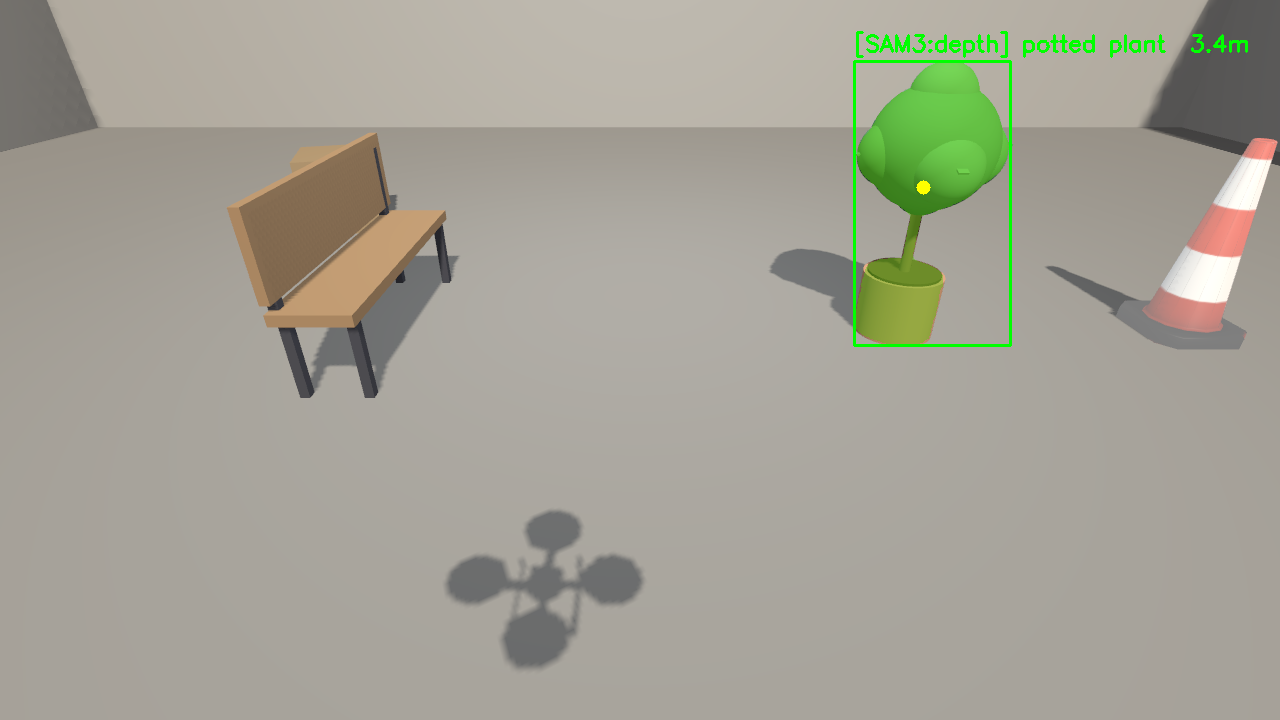
\includegraphics[width=0.95\columnwidth]{figures/sam3_detect.png}}
\caption{SAM 3 detection example. The drone has just confirmed a
\texttt{potted plant} target at score 0.85; the green overlay is
the per-pixel mask, the rectangle is the bounding box, and the
yellow dot is the centroid back-projected through the depth
camera. The text label
\texttt{[SAM3:depth] potted plant 2.0\,m} indicates the slant
range computed by the masked-depth procedure.}
\label{fig:sam3_detect}
\end{figure}

\subsection{Distance via masked depth sampling}

To convert a 2D mask into a 3D position, we sample the drone's
depth camera under the segmentation mask. A naive centroid sample
is brittle on porous objects (e.g.~plant foliage) because background
depth bleeds through gaps. We mitigate this in three steps:
\begin{enumerate}
    \item \textbf{Mask warp.} The RGB camera is $1280\times720$ and
    the depth camera $640\times480$; both share intrinsics and pose
    up to a focal-length scale. We apply a closed-form affine warp
    to project the mask into depth-image coordinates.
    \item \textbf{Erosion.} The mask is eroded by a few pixels with
    OpenCV to remove silhouette-edge bleed-through onto the
    background.
    \item \textbf{$10^{\text{th}}$-percentile aggregation.} Among
    the surviving valid depth values, we take the
    $10^{\text{th}}$ percentile rather than the median. This
    biases toward the closer surface, which is virtually always
    the actual object when the mask includes some background.
\end{enumerate}

\subsection{Bearing-only triangulation}

The estimated distance is noisy ($\sim$30--50\,cm RMS error per hit
even after the masked sampling above). To avoid relying on it,
we compute a 3D \emph{bearing ray} from the drone's pose and the
mask centroid pixel. Each detection produces a tuple
$(\mathbf{o}_i, \mathbf{d}_i)$ of ray origin and unit direction in
the world frame.

Across multiple drone positions, we solve for the world point
$\mathbf{p}^{\star}$ closest in the least-squares sense to all
rays. Each ray contributes a $3\times 3$ projection matrix
$\mathbf{P}_i = \mathbf{I} - \mathbf{d}_i \mathbf{d}_i^{\top}$
that nullifies components along the ray direction. The
constraint $\mathbf{P}_i (\mathbf{p}^{\star} - \mathbf{o}_i)
\approx \mathbf{0}$ holds approximately for each $i$, giving the
closed-form normal equations
\begin{equation}
\left(\sum_i \mathbf{P}_i\right) \mathbf{p}^{\star}
\;=\;
\sum_i \mathbf{P}_i \mathbf{o}_i
\label{eq:triangulate}
\end{equation}
which we solve directly. Crucially, this estimator depends on
\emph{ray directions only}; the noisy depth measurement is used for
fallback estimates and diagnostics but does not enter the normal
equations. We validated the formulation on synthetic data:
five rays from different vantages with $2^{\circ}$ direction noise
each produced a 33\,cm RMS error to a target at $(3, 4, 0)$.

In summary, each successful SAM 3 detection provides a mask centroid
in the image, which is back-projected into a unit bearing ray
$\hat{\mathbf{d}}_i$ in the world frame at the camera origin
$\mathbf{o}_i$. After five accepted detections from different drone
poses, the target position $\hat{\mathbf{p}}^{\star}$ is the point
closest to all rays in the least-squares sense
\eqref{eq:triangulate}. An angular-spread check (next subsection)
rejects near-parallel ray geometry and triggers a depth-projected
median fallback.

\subsection{Parallel-ray detection}

The system in \eqref{eq:triangulate} is well-conditioned only when
the rays span a meaningful angular range. For nearly-parallel rays
(drone moving in a straight line, target at a stable image
position), $\sum_i \mathbf{P}_i$ becomes singular and the
least-squares solution drifts toward the centroid of the ray
origins, which is wrong by exactly the triangulation baseline.

We detect this by computing the maximum pairwise angle between
ray directions in the cluster:
\begin{equation}
\theta_{\max} \;=\; \max_{i \ne j}
\arccos(\mathbf{d}_i \cdot \mathbf{d}_j)
\label{eq:spread}
\end{equation}
If $\theta_{\max} < 25^{\circ}$, we reject the triangulation and
fall back to the spatial median of the per-hit
distance-projected XY estimates. The threshold was tuned
empirically: in our tests, spreads below $\sim 20^{\circ}$ produced
clearly diverged solutions, while spreads above $\sim 30^{\circ}$
produced sub-meter results. We use $25^{\circ}$ as a conservative
midpoint between these regimes.

\subsection{Multi-view gate and spatial clustering}

Without care, the 20\,Hz mission timer ingests the same SAM 3
detection multiple times before the next inference fires, producing
zero-parallax duplicates. The multi-view gate requires the drone
to have moved at least 30\,cm or yawed at least $10^{\circ}$
between consecutive accepted hits.

Because SAM 3 can occasionally misidentify objects of similar shape,
we cluster hits spatially. A new hit joins the first existing
cluster whose centroid lies within 2\,m; otherwise, it spawns a
new cluster. A cluster is confirmed once it accumulates five hits,
has an average SAM 3 score of at least 0.45, and meets the
$25^{\circ}$ spread requirement. If the search exhausts without
confirming any cluster, we instead select the cluster with the
highest average SAM 3 score (with at least two hits) and triangulate
that cluster.

\section{Mission Planning and Control}
\label{sec:mission}

\texttt{mission\_node} runs an eight-state machine at 20\,Hz:
IDLE $\rightarrow$ SEARCH $\rightarrow$ APPROACH $\rightarrow$
ORBIT\_LOW $\rightarrow$ CLIMB $\rightarrow$ ORBIT\_HIGH $\rightarrow$
RETURN $\rightarrow$ LAND.

\subsection{Search trajectory}

The drone climbs to a search altitude of 1.8\,m and executes a
boustrophedon (lawnmower) sweep over four columns at
$x\in\{-3, -1, +1, +2.5\}$\,m, with $y$ alternating between
$+4$ and $-4$\,m. Search speed is 1\,m/s, intentionally slow so
that SAM 3 produces multiple frames of detection per object as the
drone passes nearby. The search waypoints are inside the room
walls with margin; the trajectory is precomputed and not reactive,
because there are no dynamic obstacles in the scene. Reactive
planning would be the natural extension for outdoor or shared
spaces.

\subsection{Approach}

When a cluster confirms, the drone heads in a straight line toward
the locked target XY at constant altitude until it is within
\texttt{orbit\_radius} + 0.3\,m horizontally. The 0.3\,m hysteresis
prevents oscillation at the boundary.

\subsection{Orbit and virtual gimbal pitch}

Both orbits are circular trajectories at the locked target XY:
\begin{equation}
\begin{aligned}
x(\phi) &= t_x + R\cos\phi, \\
y(\phi) &= t_y + R\sin\phi, \\
\text{yaw}(\phi) &= \mathrm{atan2}(t_y - y, t_x - x)
\end{aligned}
\label{eq:orbit}
\end{equation}
where $\phi$ advances at 0.15\,rad/s. The yaw line keeps the camera
rigidly pointed at the target's horizontal position.

The drone's camera is mounted with a fixed $30^{\circ}$ downward
pitch in the SDF. At ORBIT\_LOW (altitude 1.5\,m, radius
1.5\,m), this geometry naturally centers the target in the frame.
At ORBIT\_HIGH (altitude 3\,m, same radius), however, the optical
axis hits the ground at $3 / \tan(30^{\circ}) \approx 5.2$\,m
horizontally, far past the target. The target slides to the
bottom edge of the frame, and the OpenCV tracker (used during
orbit for speed) drifts to whatever stays centered (e.g.~a
nearby cone in our scene).

To address this without adding a mechanical gimbal, we introduce
a virtual gimbal: the drone body is pitched forward by the
geometric correction
\begin{equation}
\theta_{\text{pitch}} =
\mathrm{atan2}(z_{\text{drone}} - z_{\text{target}}, R)
- \theta_{\text{cam}}
\label{eq:gimbal}
\end{equation}
where $\theta_{\text{cam}} = 30^{\circ}$ is the static camera
mount angle. At ORBIT\_LOW the correction is approximately
$-2^{\circ}$ (essentially level); at ORBIT\_HIGH it is
approximately $+27^{\circ}$ (nose-down). Because the drone is
in kinematic mode, this is a quaternion-only change with no
physics implications. The pitch resets to 0 on every
non-orbit state transition.

\subsection{Image capture}

\texttt{image\_capture} buffers the camera stream and the
\texttt{/drone/pose} topic continuously. On every \texttt{Bool}
pulse on \texttt{/mission/capture} (fired every $7.5^{\circ}$ of
orbit angle by \texttt{mission\_node}), it writes the latest
frame to disk and appends the camera pose to a
\texttt{transforms.json} file in nerfstudio format and a
\texttt{poses.json} file for DA3. With a $7.5^{\circ}$ angular
step, each orbit produces 48 captures, and the two altitudes
together yield up to 96 image-pose pairs that are subsequently
used as input to the reconstruction stage.

\section{3D Reconstruction Pipeline}
\label{sec:recon}

On \texttt{MISSION COMPLETE}, \texttt{image\_capture} launches the
reconstruction pipeline as a detached subprocess so it survives
mission shutdown. The pipeline produces four output files in
\texttt{\textasciitilde/recon\_output/exports/}.

\subsection{DA3 colored point cloud}

DA3 is invoked through its CLI (\texttt{da3 auto}), which:
(1)~runs depth inference per image, (2)~jointly refines camera
extrinsics across the input frames, and (3)~fuses per-frame depth
maps into a single colored 3D point cloud. We use the
\texttt{DA3-LARGE} variant ($\sim$0.35\,B parameters), which fits
within our 8\,GB GPU memory budget; the
\texttt{DA3NESTED-GIANT-LARGE} variant (1.4\,B parameters) exceeded
the available 8\,GB memory budget and produced out-of-memory errors
in our testing. DA3's native output format is GLB (binary glTF~2.0);
we added a small \texttt{trimesh}-based conversion step to extract
the embedded point cloud and write a Stanford PLY file
(\texttt{scene\_da3.ply}). Inference takes approximately
3 minutes.

\subsection{Open3D Poisson surface reconstruction}

The DA3 cloud is then passed through Open3D's Poisson surface
reconstruction \cite{kazhdan2006poisson, zhou2018open3d}, which
estimates per-point normals and fits an implicit surface to the
point cloud. The result, written to \texttt{scene\_mesh.ply}, is a
continuous triangle mesh suitable for visual inspection and import
into 3D modeling software. Because we do not compare the mesh to
ground-truth geometry in this report, measurement accuracy should
be treated as approximate. Poisson reconstruction takes
approximately 30 seconds.

\subsection{Splatfacto 3D Gaussian Splatting}

splatfacto \cite{tancik2023nerfstudio} trains a 3DGS model on the
captured images and their poses for 30\,000 iterations
(approximately 10--15 minutes on our hardware). The trained model
is exported via \texttt{ns-export gaussian-splat} twice: once
unrestricted (\texttt{scene\_splat.ply}, the whole room) and once
restricted to a per-target axis-aligned bounding box defined in
\texttt{targets.py} (\texttt{splat\_pruned.ply}, the orbited
object only).

\subsection{Order of operations}

DA3 runs before splatfacto. The reason is VRAM management:
splatfacto's nerfstudio viewer holds approximately 4\,GB of
VRAM after training and may remain alive for user inspection; if
splatfacto ran first, DA3 (which needs roughly 3--4\,GB at
inference) could exceed the remaining headroom on the 8\,GB GPU.
With DA3 first, the DA3 subprocess fully exits and releases its
memory before splatfacto initializes. Total wall-clock per target
is approximately 15--18 minutes.

\section{User Inputs and Control Modalities}

The system accepts target prompts through four interfaces, all
of which converge on the same launch argument
\texttt{target:=<name>}:

\begin{enumerate}
    \item \textbf{Direct text} via the launch argument
    (e.g.~\texttt{ros2 launch drone\_recon scene1.launch.py
    target:="potted plant"}).
    \item \textbf{Voice}: the \texttt{voice\_mission} node records
    audio from the system microphone, transcribes it with
    faster-whisper (a quantized variant of Whisper
    \cite{radford2023whisper}), parses the intent, and calls \texttt{execvp} on
    the same launch command.
    \item \textbf{Graphical interface}: \texttt{voice\_gui}
    (Fig.~\ref{fig:voice_gui}) provides a Tkinter window with a
    microphone button and a text-fallback field for users
    without microphone access.
    \item \textbf{Free-form natural language}:
    \texttt{ai\_mission} dispatches the input through Qwen 2.5
    7B \cite{yang2024qwen25} hosted in Ollama. The LLM is presented
    with a tool schema for \texttt{start\_inspection(target)} and
    \texttt{start\_mapping()}; it returns a structured tool call
    that is converted into the launch argument vector. Qwen is
    unloaded from GPU memory before the mission launches in order
    to free VRAM for SAM 3 and DA3.
\end{enumerate}

\begin{figure}[!t]
\centerline{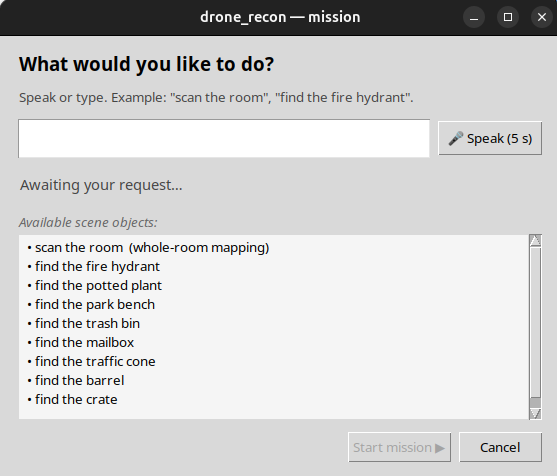
\includegraphics[width=0.85\columnwidth]{figures/voice_gui.png}}
\caption{The \texttt{voice\_gui} Tkinter frontend, showing the
text-and-voice entry box and a list of detected scene objects
that the user may target.}
\label{fig:voice_gui}
\end{figure}

\section{Scene Randomization}

To ensure every run is a genuine vision-based target-discovery
test, we shuffle which physical object occupies each canonical slot
before the drone takes off. The five canonical positions are fixed
(\,$(0,0)$, $(-3.5, 1.5)$, $(-3.5, -1.5)$, $(1.5, -2.0)$, and
$(1.5, 2.0)$\,m), but the assignment object\,$\rightarrow$\,slot is
random.

\texttt{scene\_randomizer} is a one-shot ROS\,2 node started 4\,s
after the launch. It calls \texttt{SetEntityPose} once per object
to teleport each model to its randomly-chosen canonical slot,
then exits. A \texttt{seed:=N} parameter (default 0, meaning OS
entropy) reproduces a given permutation for repeatable testing.
Critically, \texttt{mission\_node} hard-codes the
\texttt{expected\_target\_xy} field to \texttt{None}, and there is
no API by which the mission node can query an object's position.
The drone must therefore identify the named object visually for
each run rather than reading its target position from the SDF
file.

\section{Results}
\label{sec:results}

\subsection{Experimental setup}

All experiments were performed on a single workstation with an
NVIDIA mobile GPU with 8\,GB of VRAM, an AMD Ryzen-class CPU, and
32\,GB of system RAM, running Ubuntu 24.04 LTS. The robotic stack
consists of ROS\,2 Jazzy Jalisco and Gazebo Sim Harmonic
(\texttt{gz sim} 8.x), bridged through \texttt{ros\_gz\_bridge}.
The drone is a custom hand-authored X3 quadrotor model defined in
SDF, equipped with one $1280\!\times\!720$ RGB camera at 15\,Hz,
one $640\!\times\!480$ depth camera at 10\,Hz, a 360-degree GPU
LiDAR with 16 vertical channels, and an IMU. Only the RGB and depth
streams are used by the perception pipeline. The simulated room is
$20\!\times\!16$\,m with walls $3.5$\,m tall. The mission control
loop runs at 20\,Hz, and SAM 3 inference runs at approximately
2\,Hz with stride 2. Each mission captures up to 48 images per
ring across two altitudes (a low orbit at $1.5$\,m and a high
orbit at $3.0$\,m); the orbit radius is defined per target in
\texttt{targets.py} and is typically in the $1.5$--$2.0$\,m range.
End-to-end runtime per target is approximately 20 minutes:
$\sim$5 minutes for flight and capture, $\sim$3 minutes for DA3
inference, $\sim$30 seconds for Open3D Poisson meshing, and
$\sim$10--15 minutes for splatfacto training (30\,000 iterations).

The Gazebo world is hand-authored SDF, which is Gazebo's plain-XML
scene format. Off-the-shelf Gazebo Fuel community meshes were used for
the fire hydrant and construction cones, while the room walls, floor,
lighting, and four primitive replacement targets (bench, trash bin,
mailbox, and potted plant) were authored manually. The drone itself
is a custom primitive model: the design, including sensor placements,
body proportions, gimbal location, and $+$-configured propellers,
was specified by the author. Because the resulting drone block
exceeded 200 lines of repetitive XML covering body links, motor
housings, propellers, landing legs, and sensor declarations, a large
language model was used to expedite conversion of the design into
well-formed SDF. The output was then iteratively refined by hand to
address issues such as a frame-edge occlusion artifact (resolved by
relocating the camera below the body) and to tune materials for SAM 3
compatibility. The final world file is approximately 800 lines of
SDF, roughly one quarter of which is the drone model.

\subsection{Localization accuracy}

Table~\ref{tab:loc_acc} reports localization error for each of
the five targets at default positions plus a moved-plant test
(plant relocated from its default $(-3.5, 1.5)$ to $(+2.0, -3.0)$
prior to launch). All results are with the
\texttt{expected\_target\_xy = None} configuration; the drone has
zero advance knowledge of object positions.

\begin{table}[!t]
\caption{Target Localization Accuracy --- vision-based target discovery, no SDF target-position prior}
\label{tab:loc_acc}
\centering
\begin{tabular}{lcccc}
\hline
\textbf{Target} & \textbf{Actual (m)} & \textbf{Estimated (m)} & \textbf{Err.} & \textbf{Score} \\
\hline
Plant (default)  & $(-3.50,\ 1.50)$  & $(-3.66,\ 1.84)$  & 0.36\,m  & 0.85 \\
Plant (\textbf{moved}) & $(+2.00,\ -3.00)$ & $(+1.56,\ -2.19)$ & 0.92\,m  & 0.91 \\
Hydrant          & $(0.00,\ 0.00)$   & $(+0.16,\ -0.34)$ & 0.37\,m  & 0.94 \\
Trash bin        & $(+1.50,\ -2.00)$ & $(+1.39,\ -2.18)$ & \textbf{0.21\,m}  & 0.87 \\
Mailbox          & $(+1.50,\ +2.00)$ & $(+2.55,\ +2.15)$ & 1.06\,m  & 0.64 \\
Bench            & $(-3.50,\ -1.50)$ & $(-5.40,\ -1.33)$ & 1.91\,m  & 0.72 \\
\hline
\end{tabular}
\end{table}

Four of the six cases produced sub-meter localization error, and
five of six were at or below 1.06\,m, with the trash bin as the
best case at 21\,cm. The bench (1.91\,m error) and mailbox
(1.06\,m error) are the weakest cases, and three factors compound
their difficulty. First, both objects have a visually weaker
silhouette than the others: the bench is a long, thin, low-profile
slab on legs, and the mailbox is a small box on a thin post. SAM 3
confidence on these is correspondingly lower (0.72 and 0.64,
respectively) compared with 0.85--0.94 for the more volumetrically
prominent plant and hydrant. Second, both silhouettes change
substantially between viewing angles: the bench appears as a long
rectangle from the side and a thin line end-on, while the mailbox
changes apparent shape with parallax around the post. This makes the
per-frame mask centroids less consistent and increases triangulation
noise. Third, both objects are placed in regions of the room with
strong distractors---the bench near the south wall corner and the
mailbox near a traffic cone---which sometimes capture borderline
mask candidates. These observations are consistent with the broader
behavior of open-vocabulary segmentation: foundation models such as
SAM 3 perform best on objects with iconic, easily distinguishable
shapes from many viewpoints and degrade on flatter or more ambiguous
geometry. Replacing the bench primitive with a more iconic mesh
(e.g., one with visible wood grain and clearly rounded armrests) is
the highest-value asset improvement identified from these tests.

The moved-plant case is the strongest evidence for genuine
vision-only autonomy: with the plant relocated to a slot whose
assignment was not pre-registered with the mission node, the drone
still located it within 1\,m using SAM 3 segmentation and
bearing-only triangulation alone.

This evaluation is intentionally a small, controlled proof-of-concept:
five visually distinct objects (a fire hydrant, a plant, a wooden
bench, a gray trash bin, and a USPS-style mailbox) at five canonical
positions, plus one moved-object stress test. This set is sufficient
to demonstrate that the identification, triangulation, and orbit
pipeline generalizes across object classes and across positional
layouts the drone has not previously encountered, but it is not
intended as a benchmark on the diversity of scene clutter. Scaling the
evaluation to larger object sets is straightforward in software
because SAM 3 is open-vocabulary and requires no per-object retraining;
we leave such a benchmark to future work.

\subsection{Reconstruction outputs}

Fig.~\ref{fig:results_grid} shows representative reconstruction
outputs across three of the four output formats. The pruned splat
(Fig.~\ref{fig:results_grid}a) gives a target-focused 3DGS export of
the orbited fire hydrant. The full splat
(Fig.~\ref{fig:results_grid}b) includes the surrounding scene walls
and lighting. The DA3 colored point cloud
(Fig.~\ref{fig:results_grid}c) provides a coherent colored geometry
estimate that supports qualitative inspection and approximate
measurement in simulator coordinates. The Poisson mesh (not shown
for space) is a continuous triangle surface derived from the cloud
in Fig.~\ref{fig:results_grid}c. Reconstruction quality is evaluated
qualitatively in this report; quantitative geometry metrics such as
mesh-to-ground-truth error, Chamfer distance, PSNR, and SSIM are
left for future evaluation.

\begin{figure*}[!t]
\centering
\begin{subfigure}[b]{0.32\textwidth}
    \centering
    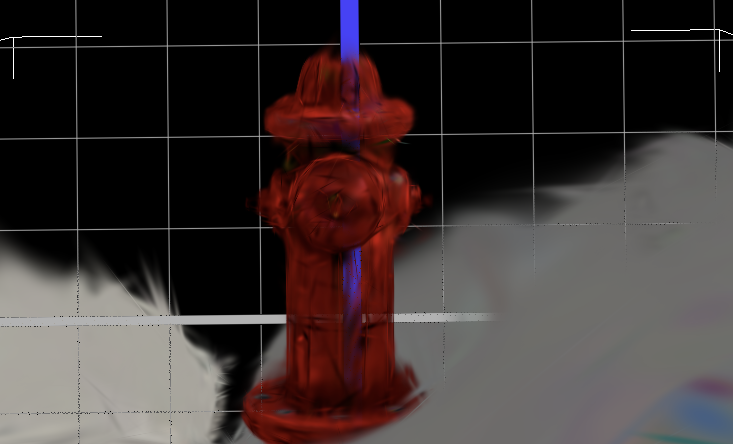
\includegraphics[width=\linewidth]{figures/splat_pruned.png}
    \caption{\texttt{splat\_pruned.ply} (3DGS, target only)}
    \label{fig:res_a}
\end{subfigure}
\hfill
\begin{subfigure}[b]{0.32\textwidth}
    \centering
    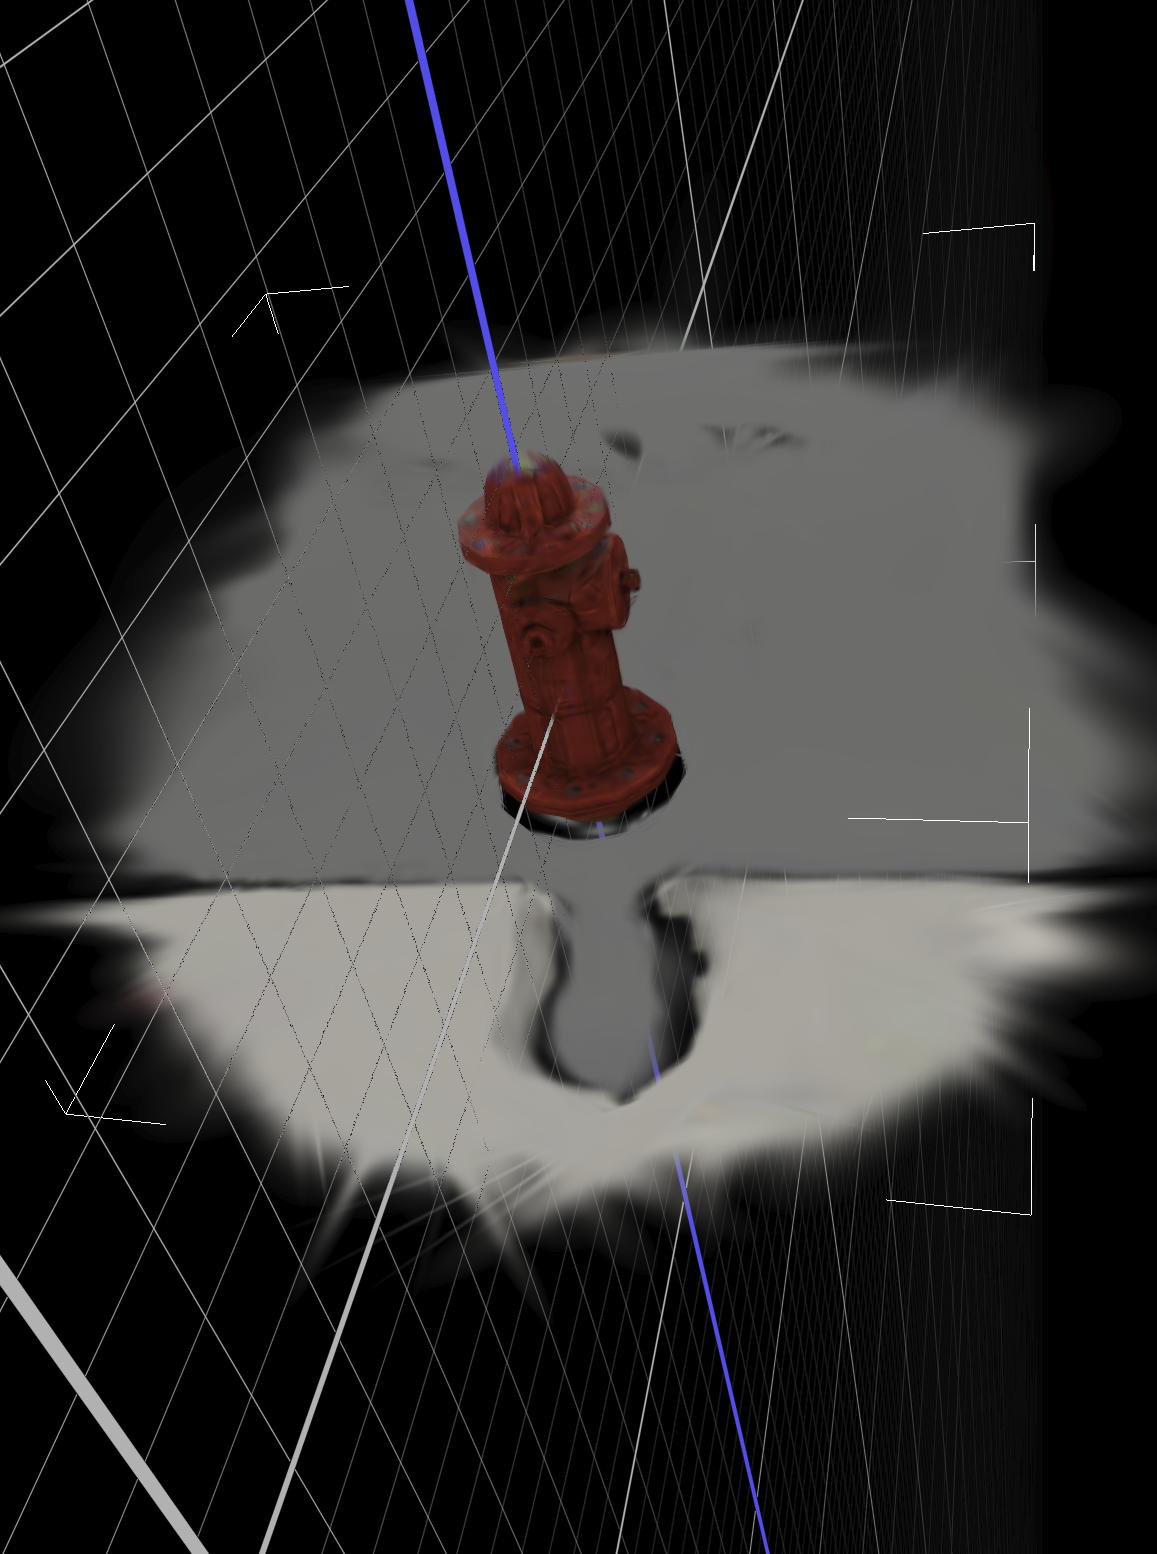
\includegraphics[width=\linewidth]{figures/splat_full.png}
    \caption{\texttt{scene\_splat.ply} (3DGS, full scene)}
    \label{fig:res_b}
\end{subfigure}
\hfill
\begin{subfigure}[b]{0.32\textwidth}
    \centering
    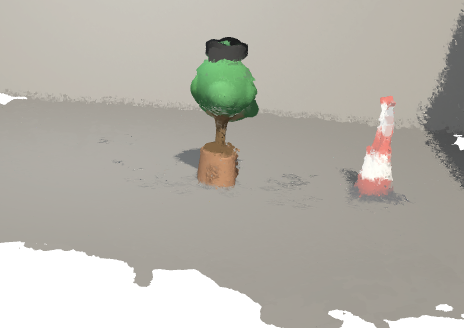
\includegraphics[width=\linewidth]{figures/da3_cloud_plant.png}
    \caption{\texttt{scene\_da3.ply} (DA3 colored point cloud)}
    \label{fig:res_c}
\end{subfigure}
\caption{Representative reconstruction outputs after one
mission. The pruned splat (a) and the full-scene splat (b) come
from the same splatfacto training run but use different export
bounding boxes. The point cloud (c) is the DA3 multi-view depth
fusion result, used as input to the Poisson surface mesh.}
\label{fig:results_grid}
\end{figure*}

\subsection{Reconstruction evaluation methodology}

Reconstruction outputs in this work are evaluated \emph{qualitatively}
through visual inspection of the four exported PLY files and
side-by-side comparison with the rendered Gazebo scene. We do not
report quantitative reconstruction metrics because the simulator does
not directly export a per-object ground-truth triangle mesh in the
same coordinate frame as the captured camera poses, and constructing
one would itself introduce alignment error. Future work should add
objective metrics including \emph{Chamfer distance} between the DA3
cloud and a sampled ground-truth mesh, \emph{point-to-mesh distance}
between the Poisson mesh and the SDF geometry, and \emph{PSNR/SSIM}
between renders of the trained 3DGS model and held-out test views
captured at unseen orbit angles. We report localization accuracy
quantitatively (Table~\ref{tab:loc_acc}) because that metric does not
require an aligned ground-truth mesh.

\subsection{Live diagnostic view}

Fig.~\ref{fig:live_view} shows the custom \texttt{live\_view}
node during ORBIT\_HIGH. The drone is locked on a relocated
\texttt{potted plant}; the lightweight OpenCV tracker has the
target boxed in cyan with a label
\texttt{[TRK:depth] potted plant}. The status bar at the bottom
reports the current state, framerate, and source.

\begin{figure}[!t]
\centerline{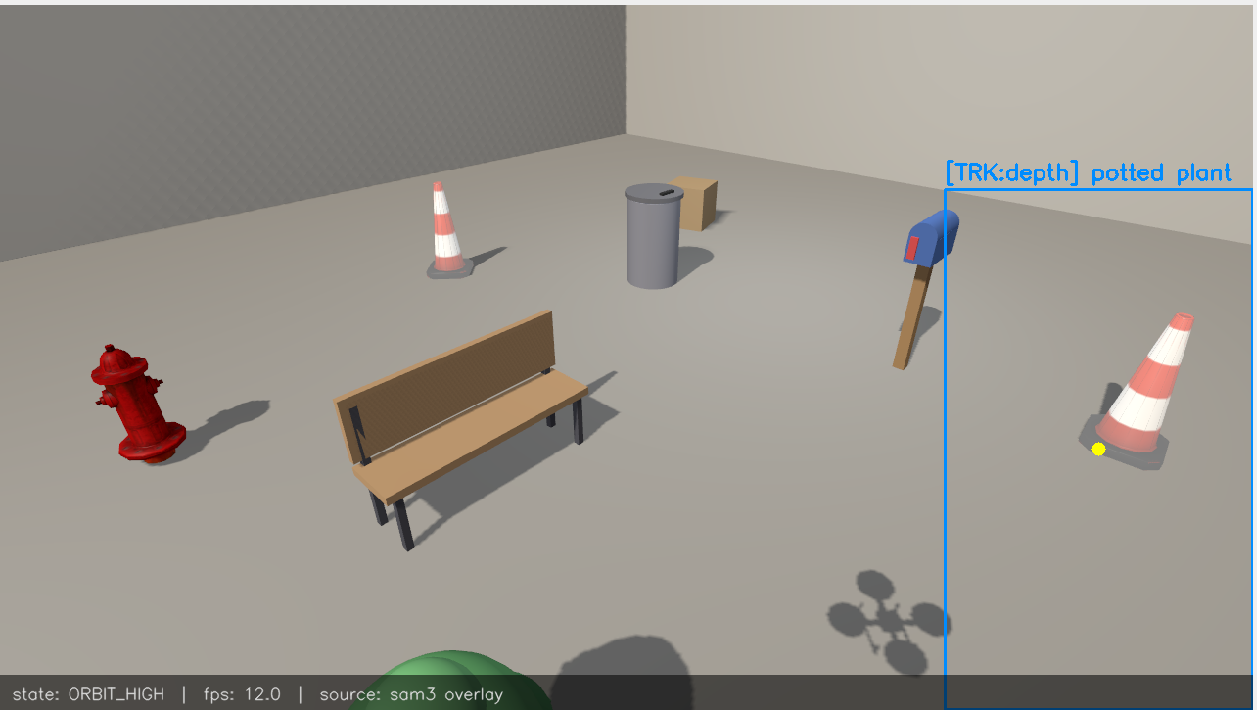
\includegraphics[width=0.95\columnwidth]{figures/live_view.png}}
\caption{Custom \texttt{live\_view} window during ORBIT\_HIGH on
the \texttt{potted plant} target. The cyan box is the OpenCV
tracker output (used during orbit for speed because SAM 3 is too
slow for this state). The status bar reports the state machine
phase, FPS, and detection source. The visible scene contains five
distractor objects: hydrant, bench, trash bin, mailbox, and a
traffic cone.}
\label{fig:live_view}
\end{figure}

\subsection{Empirical photorealism check}

The reviewer expressed concern that Gazebo's rendering quality may
not be sufficient for SAM 3. Our results indicate that this concern
is manageable in our controlled scene, though not negligible. With
the final asset set, observed SAM 3 confidence scores were 0.85
(plant), 0.94 (hydrant), 0.87 (bin), 0.64 (mailbox), and 0.72
(bench), all above the 0.30 detection threshold. However, three
Gazebo-Fuel meshes (AirportBench, TrashBin, Mailbox) did \emph{not}
register reliably in preliminary tests and were replaced with
primitive geometries constructed from boxes and cylinders. This
supports the narrower conclusion that Gazebo can be sufficient for
this pipeline when visual assets are selected or simplified
carefully; it does not imply that arbitrary Gazebo assets will work
out of the box.

\subsection{Failure modes and recovery}

Fig.~\ref{fig:failure} shows an early splat output where the
target localization triangulation diverged due to insufficient
ray spread. The result is a strongly-distorted splat with
floater artifacts: the orbit was off-center by approximately
1.5\,m, and the captured frames looked at empty space for a
substantial fraction of the orbit. We addressed this with the
$25^{\circ}$ angular-spread gate (Section~\ref{sec:vision}) and
the score-weighted cluster selection. After the fix, no
subsequent test exhibited this failure mode.

\begin{figure}[!t]
\centerline{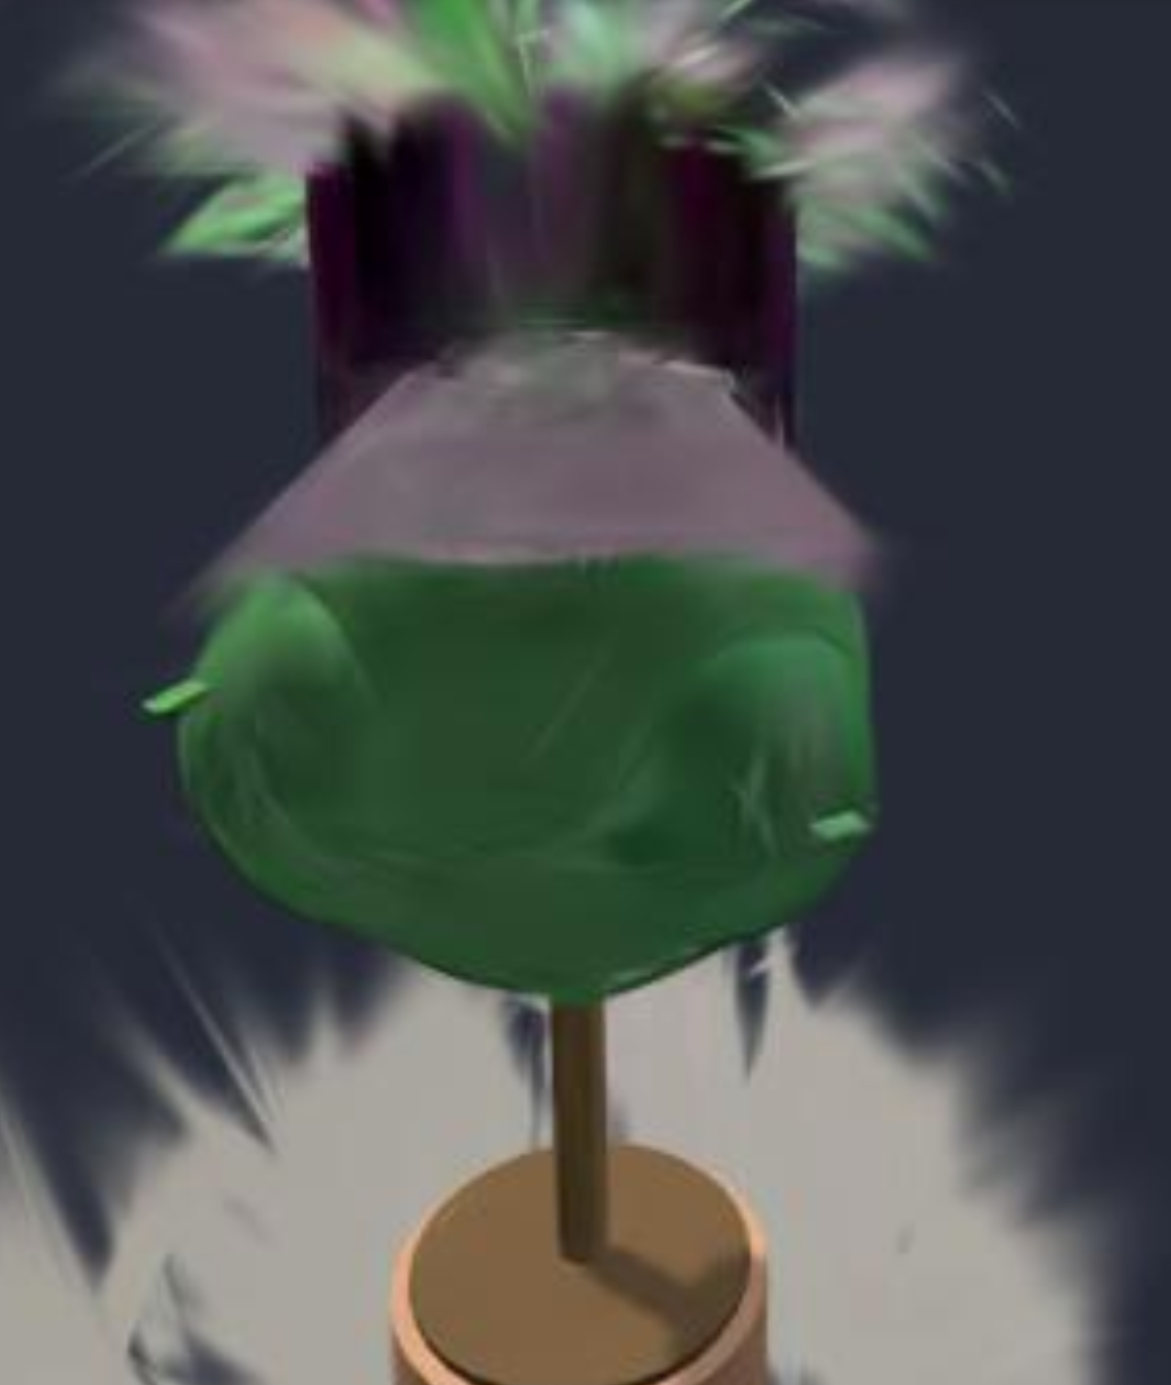
\includegraphics[width=0.65\columnwidth]{figures/failure_floaters.png}}
\caption{An early failure: the triangulation diverged on
near-parallel rays during a fast initial test, producing an
off-center orbit and a splat with significant floater artifacts.
The $25^{\circ}$ angular-spread gate and parallel-ray fallback
introduced afterward prevented this failure in subsequent tests.}
\label{fig:failure}
\end{figure}

\subsection{Ablation: effect of key design decisions}

We did not run a formal ablation study, but the practical effect of
three key design choices was directly observed during development:
\begin{itemize}
    \item \textbf{Without the $25^{\circ}$ angular-spread gate},
    the bearing-only triangulation in \eqref{eq:triangulate}
    consistently diverged when SAM 3 hits arrived from a column of
    nearly collinear drone positions. The least-squares matrix
    $\sum_i \mathbf{P}_i$ became ill-conditioned and the estimate
    drifted to the centroid of the ray origins. We observed
    orbit-center errors of $1.5$--$2.0$\,m before introducing the
    gate, followed by sub-meter errors in the successful cases after
    the gate was added.
    \item \textbf{Without the virtual gimbal pitch
    \eqref{eq:gimbal}}, the OpenCV tracker reliably drifted during
    ORBIT\_HIGH because the target slid to the bottom edge of the
    frame and the tracker locked onto whichever distractor object
    remained near image center, typically a traffic cone in our scene.
    After introducing the virtual gimbal, the target stayed near
    image center for the full orbit and tracker drift was not observed
    in subsequent tests.
    \item \textbf{Without scene randomization}, an implementation bug
    or convenience shortcut---such as caching an
    \texttt{expected\_position} from \texttt{targets.py} as a
    fallback---could silently leak SDF position priors into the
    runtime path without producing visible failures. By forcing a new
    permutation at every launch, any such regression would
    immediately manifest as the drone flying to the wrong place and
    failing to confirm the target.
\end{itemize}

\subsection{Comparison to alternative simulators}

Table~\ref{tab:sims} summarizes why Gazebo was selected for this
implementation. The comparison is qualitative and specific to the
available hardware and project goals, not a general ranking of
simulators.

\begin{table}[!t]
\caption{Simulator comparison for this project (qualitative)}
\label{tab:sims}
\centering
\resizebox{\columnwidth}{!}{%
\begin{tabular}{lccc}
\hline
\textbf{Requirement} & \textbf{Gazebo} & \textbf{Isaac Sim} & \textbf{AirSim} \\
\hline
ROS\,2 workflow & first-class & available bridge & wrapper-based \\
Cost/source model & free/open & closed NVIDIA stack & free/open \\
Rendering & sufficient here & stronger, GPU-heavy & Unreal-based \\
Scene authoring & SDF/XML & USD & Unreal project \\
Deterministic pose control & simple & possible, heavier & possible \\
8\,GB GPU practicality & yes & poor for current 5.1 specs & yes \\
Maintenance status & active & active & latest official release 2022 \\
\hline
\end{tabular}}
\end{table}

\subsection{Reproducibility}

A full mission is reproducible from a single launch command:
\begin{verbatim}
ros2 launch drone_recon scene1.launch.py \
     target:="potted plant" seed:=42
\end{verbatim}
The \texttt{seed:=N} parameter, where \texttt{N} is any non-zero
integer, makes \texttt{scene\_randomizer} produce a deterministic
permutation, so the same launch with the same seed re-runs the same
physical layout. Outputs are written to
\texttt{\textasciitilde/recon\_output/exports/} as four PLY files:
\texttt{splat\_pruned.ply}, \texttt{scene\_splat.ply},
\texttt{scene\_da3.ply}, and \texttt{scene\_mesh.ply}. The captured
images and camera-pose JSON are written to
\texttt{\textasciitilde/recon\_output/}, and the per-tick CSV flight
log is written to \texttt{\textasciitilde/flight\_logs/}. SAM 3 debug
images for the first ten detections are saved to
\texttt{/tmp/sam3\_dbg/} for visual verification of identification
quality. All source code, the world SDF, and the \texttt{targets.py}
configuration are versioned under
\texttt{\textasciitilde/ros2\_ws/src/drone\_recon/}.

\section{Discussion}

\subsection{Why bearing-only triangulation suits this task}

The masked depth measurement carries roughly 30--50\,cm RMS noise
even after the cleaning steps described above. Multiplying that
noisy distance by a ray direction propagates the error into the
final XY estimate. The bearing-only formulation in
\eqref{eq:triangulate} exploits the fact that the mask-centroid
direction is much less noisy than the sampled depth value in our
setup: the angular error of a SAM 3 mask centroid is small compared
with the fractional-meter error observed in depth sampling. Trading
noisy distance for cleaner direction is the key insight. The method
has been used for decades in bearing-only target tracking
\cite{nardone1981bearing}, sonar, and astronomical observation.

\subsection{Why we did not use SAM 3D}

A reviewer suggested SAM 3D from Meta (released 2025), which
generates a 3D shape estimate from a single image and segmentation
mask. Our use case differs in that the orbit produces multiple
calibrated views per target, so multi-view geometry can exploit
these additional observations using known simulator poses. SAM 3D's
single-view output would still be useful as a per-frame shape prior
to regularize splatfacto, and we suggest this integration as a
future extension.

\subsection{Limitations}

We clarify the precise scope of the autonomy claim: the system is
fully autonomous with respect to \emph{target discovery},
\emph{mission execution}, and \emph{multi-view image capture}; it is
\emph{not} fully autonomous with respect to vehicle self-localization,
because the drone reads its own world pose from Gazebo's ground-truth
state rather than estimating it from onboard SLAM. Adding a visual-SLAM
front end such as ORB-SLAM3 or VINS-Mono is the natural next step for
hardware deployment and would not require changes to the perception,
planning, or reconstruction stages of the pipeline.

The pipeline assumes a static, indoor, single-target inspection
task. The lawnmower search trajectory does not adapt to obstacles
because the simulated room is empty along the search corridors;
hardware deployment would need a costmap-based planner. The
kinematic pose-control mode improves reconstruction repeatability
but is not a physically realistic controller. Reconstruction
quality is shown qualitatively rather than with ground-truth
geometry metrics; future work should report Chamfer distance,
mesh-to-model error, point-cloud completeness, and image-rendering
metrics such as PSNR and SSIM where applicable. The bench primitive
remains the weakest target for SAM 3 recognition and localization,
showing that target geometry and visual distinctiveness still
matter. Finally, splatfacto training remains the longest single
step at approximately 10--15 minutes per target on an 8\,GB GPU;
faster 3DGS variants such as 3DGS-MCMC \cite{kheradmand2024_3dgs_mcmc}
could reduce this.

\section{Conclusion}

We presented an autonomous simulated UAV target-inspection pipeline
that, given only the natural-language name of a target object,
visually finds the object under an unknown object-to-slot assignment
and produces four 3D representations in approximately 20 minutes per
target. The system uses no fiducial markers and no target-position
prior, although it does rely on Gazebo's ground-truth vehicle pose
for self-localization in simulation. Scene randomization and the
moved-target test support the claim that target discovery is
vision-based. The work evolved from an AprilTag\,/\,COLMAP proposal
into a SAM 3\,/\,DA3\,/\,splatfacto hybrid, addressing the
simulator-photorealism concern through careful asset selection and
demonstrating reliable SAM 3 inference on the selected Gazebo
\texttt{ogre2} assets. The bearing-only triangulation primitive,
combined with a $25^{\circ}$ angular-spread gate, is the central
technical contribution: it separates the cleaner angular signal
from the noisier depth signal and provides a principled fallback
when the geometry is degenerate.

Future work includes replacing kinematic pose control with a PX4
velocity controller for hardware deployment, integrating SAM 3D
as a per-frame shape prior to regularize splatfacto, adopting
adaptive view planning to reduce the fixed image budget, and
performing a real-drone evaluation in an indoor arena.

\section*{Acknowledgment}

The author thanks the instructor and TAs of the
Intelligent Mobile Robotics class at Binghamton University for
project guidance and review feedback that motivated several of
the design decisions reported here, particularly the move from
fiducial-based detection to open-vocabulary segmentation.

\begin{thebibliography}{00}

\bibitem{olson2011apriltag}
E.~Olson, ``AprilTag: A robust and flexible visual fiducial
system,'' in \emph{Proc.\ IEEE Int.\ Conf.\ Robotics and
Automation}, 2011, pp.~3400--3407.

\bibitem{wang2016apriltag2}
J.~Wang and E.~Olson, ``AprilTag 2: Efficient and robust fiducial
detection,'' in \emph{Proc.\ IEEE/RSJ Int.\ Conf.\ Intelligent
Robots and Systems}, 2016, pp.~4193--4198.

\bibitem{schonberger2016sfm}
J.~L. Sch\"onberger and J.~M. Frahm, ``Structure-from-motion
revisited,'' in \emph{Proc.\ IEEE Conf.\ Computer Vision and
Pattern Recognition}, 2016, pp.~4104--4113.

\bibitem{schonberger2016mvs}
J.~L. Sch\"onberger, E.~Zheng, M.~Pollefeys, and J.~M. Frahm,
``Pixelwise view selection for unstructured multi-view stereo,''
in \emph{Proc.\ Eur.\ Conf.\ Computer Vision}, 2016, pp.~501--518.

\bibitem{kirillov2023sam}
A.~Kirillov \emph{et al.}, ``Segment anything,'' in \emph{Proc.\ IEEE/CVF
Int.\ Conf.\ Computer Vision (ICCV)}, 2023, pp.~4015--4026.

\bibitem{carion2025sam3}
N.~Carion \emph{et al.}, ``SAM 3: Segment anything with concepts,''
\emph{arXiv:2511.16719}, 2025.

\bibitem{kerbl2023_3dgs}
B.~Kerbl, G.~Kopanas, T.~Leimk\"uhler, and G.~Drettakis,
``3D Gaussian splatting for real-time radiance field rendering,''
\emph{ACM Trans.\ Graph.}, vol.~42, no.~4, 2023.

\bibitem{tancik2023nerfstudio}
M.~Tancik \emph{et al.}, ``Nerfstudio: A modular framework for neural
radiance field development,'' in \emph{ACM SIGGRAPH 2023 Conf.\
Proc.}, 2023.

\bibitem{yang2024depthanything}
L.~Yang \emph{et al.}, ``Depth Anything: Unleashing the power of
large-scale unlabeled data,'' in \emph{Proc.\ IEEE/CVF Conf.\
Computer Vision and Pattern Recognition}, 2024, pp.~10371--10381.

\bibitem{lin2025da3}
H.~Lin, S.~Chen, J.~H. Liew, D.~Y. Chen, Z.~Li, G.~Shi, J.~Feng,
and B.~Kang, ``Depth Anything 3: Recovering the visual space from
any views,'' \emph{arXiv:2511.10647}, 2025.

\bibitem{macenski2022ros2}
S.~Macenski, T.~Foote, B.~Gerkey, C.~Lalancette, and W.~Woodall,
``Robot operating system 2: Design, architecture, and uses in the
wild,'' \emph{Sci.\ Robot.}, vol.~7, no.~66, 2022.

\bibitem{koenig2004gazebo}
N.~Koenig and A.~Howard, ``Design and use paradigms for Gazebo,
an open-source multi-robot simulator,'' in \emph{Proc.\ IEEE/RSJ
Int.\ Conf.\ Intelligent Robots and Systems}, 2004,
pp.~2149--2154.

\bibitem{nvidia_isaac_req}
NVIDIA, ``Isaac Sim requirements,'' \emph{Isaac Sim Documentation},
2026. [Online]. Available: \url{https://docs.isaacsim.omniverse.nvidia.com/5.1.0/installation/requirements.html}

\bibitem{airsim_releases}
Microsoft, ``Releases: microsoft/AirSim,'' GitHub repository, latest
official release v1.8.1, 2022. [Online]. Available:
\url{https://github.com/microsoft/AirSim/releases}

\bibitem{mildenhall2020nerf}
B.~Mildenhall \emph{et al.}, ``NeRF: Representing scenes as neural
radiance fields for view synthesis,'' in \emph{Proc.\ Eur.\ Conf.\
Computer Vision}, 2020, pp.~405--421.

\bibitem{kazhdan2006poisson}
M.~Kazhdan, M.~Bolitho, and H.~Hoppe, ``Poisson surface
reconstruction,'' in \emph{Proc.\ Eurographics Symp.\ Geometry
Processing}, 2006, pp.~61--70.

\bibitem{zhou2018open3d}
Q.-Y. Zhou, J.~Park, and V.~Koltun, ``Open3D: A modern library for
3D data processing,'' \emph{arXiv:1801.09847}, 2018.

\bibitem{radford2023whisper}
A.~Radford \emph{et al.}, ``Robust speech recognition via large-scale
weak supervision,'' in \emph{Int.\ Conf.\ Machine Learning}, 2023.

\bibitem{yang2024qwen25}
A.~Yang \emph{et al.}, ``Qwen2.5 technical report,''
\emph{arXiv:2412.15115}, 2024.

\bibitem{zhang2020uav_planning}
S.~Zhang, C.~Liu, and N.~Haala, ``Three-dimensional path planning
of UAVs imaging for complete photogrammetric reconstruction,''
\emph{ISPRS Annals of the Photogrammetry, Remote Sensing and
Spatial Information Sciences}, vol.~V-1-2020, pp.~325--331, 2020.

\bibitem{smith2018adaptive_view}
N.~Smith, N.~Moehrle, M.~Goesele, and W.~Heidrich, ``Aerial path
planning for urban scene reconstruction: A continuous optimization
method and benchmark,'' \emph{ACM Trans.\ Graph.}, vol.~37, no.~6,
2018.

\bibitem{nardone1981bearing}
S.~C. Nardone and V.~J. Aidala, ``Observability criteria for
bearings-only target motion analysis,'' \emph{IEEE Trans.\
Aerospace and Electronic Systems}, vol.~AES-17, no.~2,
pp.~162--166, 1981.

\bibitem{kheradmand2024_3dgs_mcmc}
S.~Kheradmand \emph{et al.}, ``3D Gaussian splatting as Markov
chain Monte Carlo,'' in \emph{Advances in Neural Information
Processing Systems}, 2024.

\bibitem{gallai_proposal_2026}
M.~Gallai, ``Autonomous sim drone for target orbit imaging and 3D
reconstruction,'' Project Proposal, Intelligent Mobile Robotics,
Binghamton University, March 2026.

\end{thebibliography}

\end{document}
